\documentclass[12pt, a4papre]{article}
\usepackage[catalan]{babel}
\usepackage[unicode]{hyperref}
\usepackage{amsmath}
\usepackage{amssymb}
\usepackage{amsthm}
\usepackage{xifthen}
\usepackage{siunitx}
\usepackage{xcolor}
\usepackage{float}
\usepackage{listings}
\usepackage{setspace}
\usepackage{graphicx}
\usepackage{tikz,lipsum,lmodern}
\usepackage[most]{tcolorbox}
\usepackage{circuitikz}
\usepackage{indentfirst}
\usepackage{verbatimbox}
\definecolor{mygreen}{RGB}{28,172,0} % color values Red, Green, Blue
\definecolor{mylilas}{RGB}{170,55,241}
\graphicspath{ {./images/} }

\hypersetup{
    colorlinks = true,
    linkcolor = blue
}

\author{	
		Igor Yuziv\\
		Edison Gabriel Zaragosin\\
		Oriol Torres\\
		Albert Tomas\\
		Daniel Vilardell}
\newpage

\title{\textbf{\textcolor{blue}{ENTIC-lab\\
	Answers to WP questions}}}
\date{2020-2021}

\begin{document}

	\lstset{language=Matlab,%
		frame=single,  
    		%basicstyle=\color{red},
    		breaklines=true,%
    		morekeywords={matlab2tikz},
    		keywordstyle=\color{blue},%
    		morekeywords=[2]{1}, keywordstyle=[2]{\color{black}},
   		 identifierstyle=\color{black},%
    		stringstyle=\color{mylilas},
    		commentstyle=\color{mygreen},%
    		showstringspaces=false,%without this there will be a symbol in the places where there is a space
    		numbers=left,%
    		numberstyle={\tiny \color{black}},% size of the numbers
    		numbersep=9pt, % this defines how far the numbers are from the text
    		emph=[1]{for,end,break},emphstyle=[1]\color{red}, %some words to emphasise
    		%emph=[2]{word1,word2}, emphstyle=[2]{style},    
	}
	
	\maketitle
	\newpage
	\begin{center}
	\footnotesize{
		Before doing any certain task, the related questions must be answered in this file.
		
		\textcolor{red}{You must update this file as many times as necessary with the format WPAnswers\_g\_t.pdf}
		
 		(Keep the Atenea task in draft status until you finish the Lab-Project part A)
		}
	\end{center}

	\textcolor{blue}{Question 0.1:} \textbf{How often must you deliver a Gantt Diagram updated version?}
	\begin{itemize}
		\item At the beginning of each WP
		\item \textcolor{red}{ \textbf{Each lab session}}
		\item At the beginning and at the end of Parts A and B
	\end{itemize}
	
	\textcolor{blue}{Question 0.2:} \textbf{If you are the team 7 of subgroup 63, which is the right filename for deliver the Final Report in Atenea at the end of the semester? What is the deadline day for deliver this document?}
	
	The filename would have to be FinalReport\_63\_7 and the deadline for this document to be delivered is 14/01/2021.
	
	\textcolor{blue}{Question 0.3:} \textbf{What penalization will have you if you deliver a document one week later?}
	\begin{itemize}
		\item 15\%
		\item \textcolor{red}{ \textbf{30\%}}
		\item 50\%
	\end{itemize}
	
	\textcolor{blue}{Question 0.4:} \textbf{When you must deliver the Answers to the WP questions?}
	\begin{itemize}
		\item At the beginning of each WP
		\item At the end of each Part
		\item \textcolor{red}{ \textbf{Continuously during the semester, when you need the answer of each question\%}}
	\end{itemize}
	
	\textcolor{blue}{Question 0.5:} \textbf{How you plan to avoid the “Hitchhiker and Couch Potatoes” in your team?}
	
	In order to avoid the “Hitchhiker and Couch Potatoes” in our team, what we will do is to make sure that there is good communication between us and that we all understand what our task is and what we are doing at all times. If in any case there were a problem, the teacher would be notified quickly in order to solve it as soon as possible.
	
	\newpage
	
	\section{WP1 - Mechanical}
	\textcolor{blue}{Question 1.1:} \textbf{Calculate how much additional weight is necessary if the holes are not made in the ROUV elbows PVC structure. Inner diameter of PVC pipe: 16 mm.}
	
	We can calculate the total volume with the folowing formula
	
	\[
		\text{Total volume} = \text{\#Tubes}\cdot\pi r^2 l
	\]
	
	Then we find the weight for each group of tubes
	
	\[
		8\cdot \pi \cdot0.8^2\cdot 15 = 241.27 cm^3
	\]
	\[
		2\cdot \pi \cdot0.8^2\cdot 10 = 40.21 cm^3
	\]
	\[
		4\cdot \pi \cdot0.8^2\cdot 5 = 40.21 cm^3
	\]
	
	Then using a conversion factor we can calculate the total weight with the sum of the previously calculated volume, $241.27 + 40.21 + 40.21 = 321.69 cm^3$.
	\[
		\text{Weight} = 321.69cm^3\cdot \frac{1dm^3}{1000cm^3}\cdot \frac{1m^3}{1000dm^3}\cdot \frac{1kg}{1dm}\cdot \frac{1000g}{1kg} = 0.321 g
	\]
	
	\textcolor{blue}{Question 1.2:} \textbf{Which is the maximum voltage applicable to the electrical motor? Which current is demanded by the motor at the maximum speed?}
	
	The maximum voltage aplicable to the electrical motor is 12V and the current by the motor at maximum speed is $2.5A$.\\
	\newpage
	\textcolor{blue}{Question 1.3:} \textbf{Include a picture of the initial and final Gantt diagrams of WP1, making a reflexion about the progress and explaining any delay in the development of the tasks.}
	
	\begin{figure}[H]
		\begin{center}
		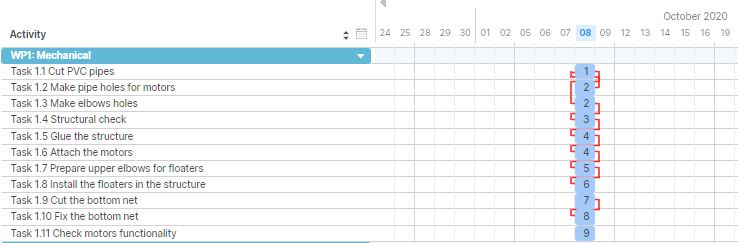
\includegraphics[width=150mm]{WP1-1-10-2020.jpg}
		\end{center}
	\end{figure}
	
	The last task had to be delayed due to not having enough time to complete it. We wasted more time than necessary fixing an error during assembly. But finally everything worked out correctly.

	
	\newpage
	\section{WP2 - Electrical} 
	
	\textcolor{blue}{Question 2.1:} \textbf{In the market there are different types of switches. Which type among the switch models shown in Fig. 2.2 are we using in this project?}
	
	We are going to use a DPDT switch because the motor is just compatible with it.\\
	
	\textcolor{blue}{Question 2.2:} \textbf{The ROUV motors are the core of nautical bilge pumps Johnson L450 model (specifications are available in ATENEA Support Documents section). Which is the electrical power required for one ROUV motor? Calculate the total electrical power the ROUV battery must supply. Which is the fuse value in your stock material? What are you protecting with this fuse?}
	
	According given datasheet L450: $V=12$ , $I=2.5$. We will use three motors to have X3 power than before.
	
	\[
		P = 3VI = 3\cdot12\cdot 2.5 = 90W
	\]
	
	The value of the fuse in our stock material is 5A acording to the manual given. With this fuse we are protecting the cirquit from getting overloads or overcurrents.

	\textcolor{blue}{Question 2.3:} \textbf{You must make some soldering to electrically connect different parts of your vehicle. You can watch some videos in YouTube about how to solder like, for example, \url{https://youtu.be/xrVCkEoY_8M} . Which is the use of the sponge we have in the solder holder?}
	
	Sponge is used to clean soldering tip when it is hot, cleaning is so important to make a strong welders.\\
	\newpage
	\textcolor{blue}{Question 2.4:} \textbf{Now it is time to make all the connections with the flexible wires inside the box to control the ROUV motors. Draw a sketch of the complete electrical circuit using the CAD schematic software https://www.tinycad.net/. In ATENEA Support Documents section an specific library for ENTIC is available. If you need more information to do this, you can search images in internet about “DPDT motor”.}
	
	\begin{figure}[H]
		\begin{center}
		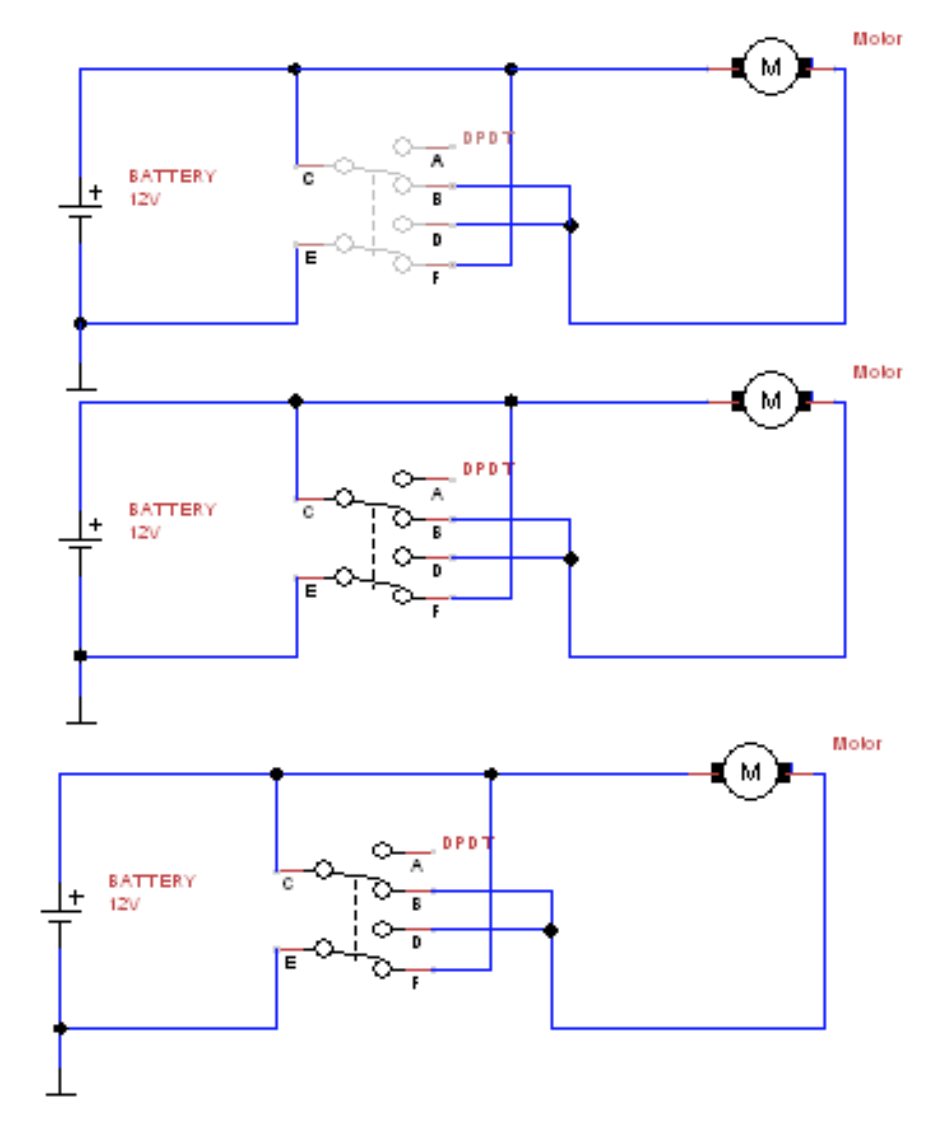
\includegraphics[width=80mm]{Cirquit1WP2.png}
		\end{center}
	\end{figure}
	
	\newpage
	\textcolor{blue}{Question 2.5:} \textbf{Update yoursketch of the electrical circuit (include the fuse and the DB9 connector)}
	
	\begin{figure}[H]
		\begin{center}
		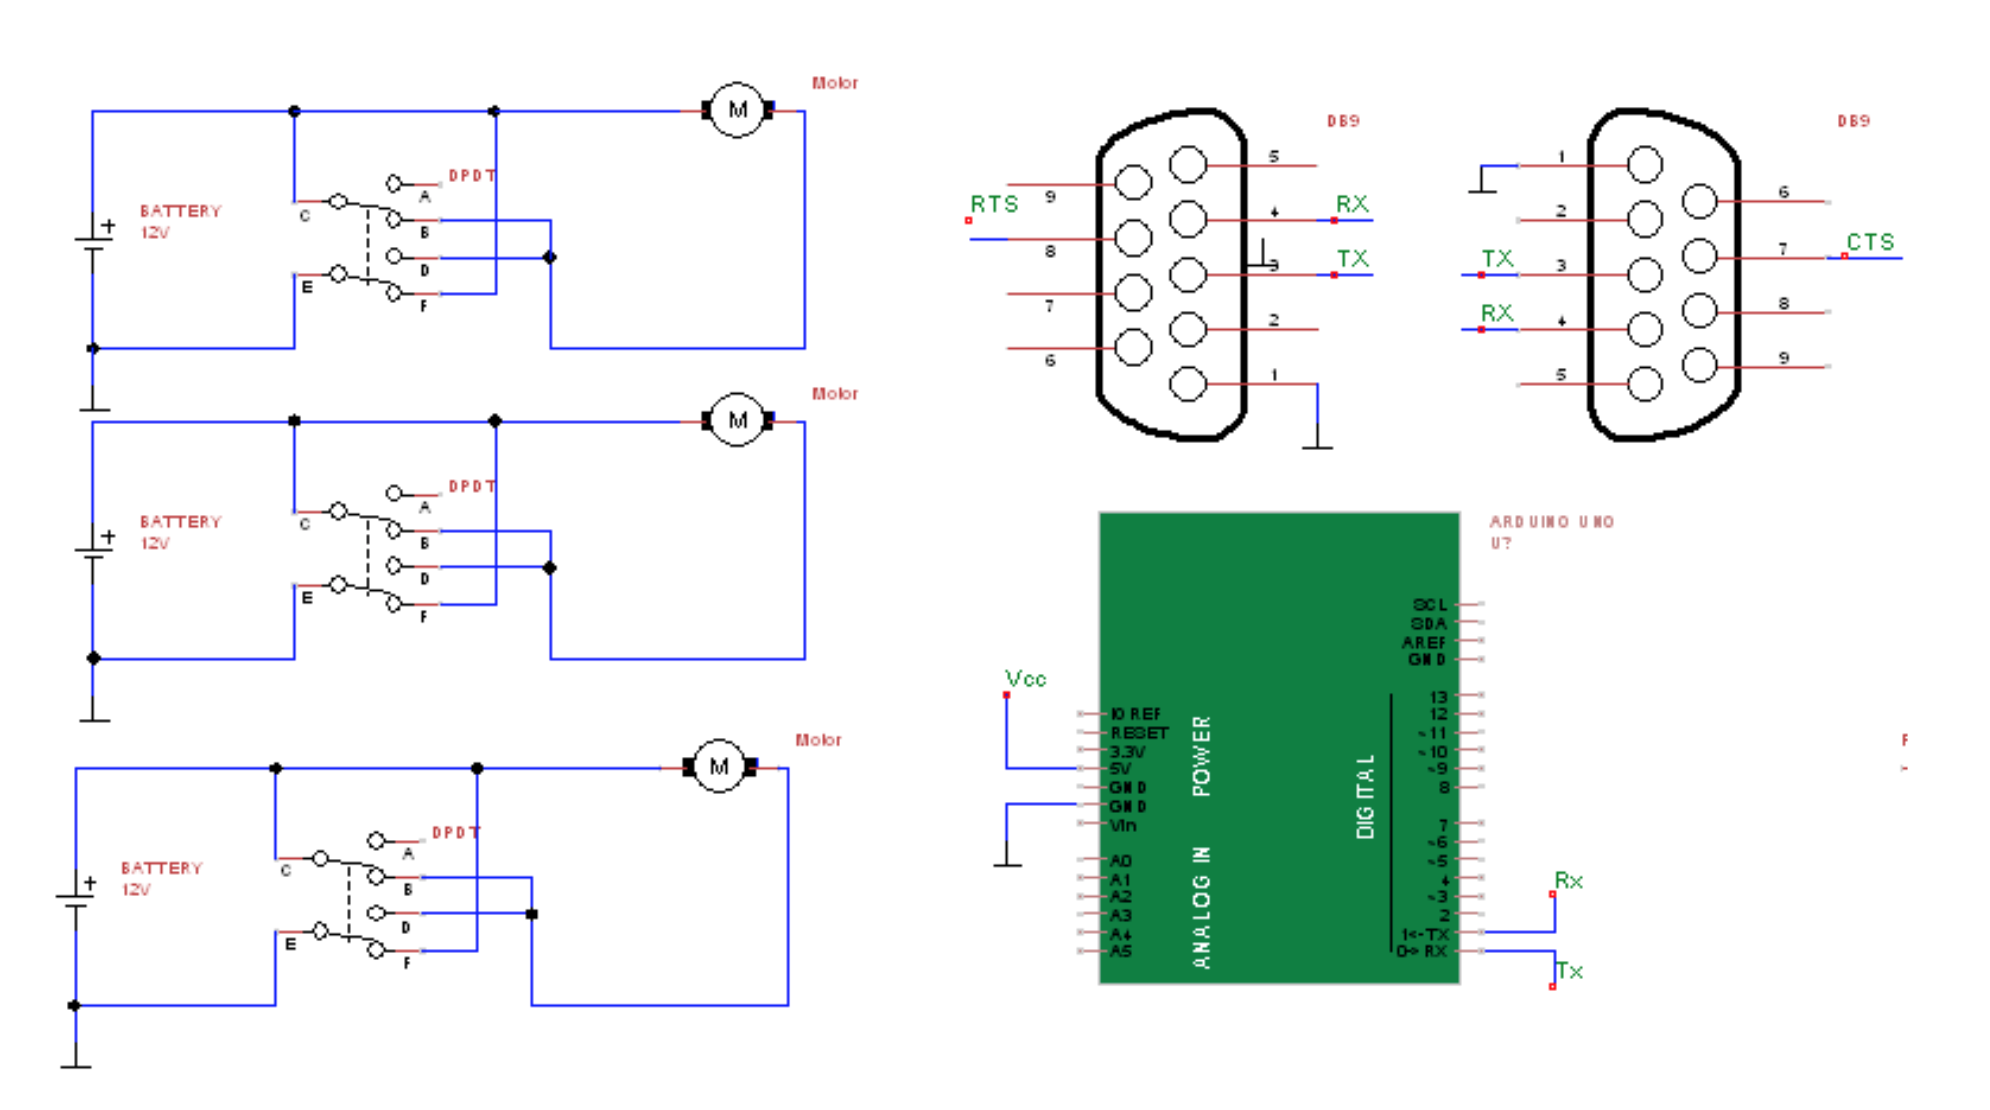
\includegraphics[width=150mm]{Cirquit2WP2.png}
		\end{center}
	\end{figure}
	
	\newpage
	\section{WP3 - Electronics}

	\textcolor{blue}{Question 3.1:} \textbf{Which pressure increase will be observed at 3 m depth?}
	\[
		0.986\cdot\frac{3}{10} = 0.2958 Atm
	\]

	\textcolor{blue}{Question 3.2:} \textbf{Will this pressure depend or not on the atmospheric pressure at water surface? Why?}\\
	
		If what we want is to calculate the real pressure that will be exerted on the ROUV, we must also take into account the atmospheric pressure on the surface. On the other hand, if what we want is only to calculate the increase with respect of this, it will not be necessary.\\
	
	\textcolor{blue}{Question 3.3:} \textbf{Analyse the circuit of Fig. 4.2 and obtain the output voltage VS. Then, find the dependence of VS on the relative variation due to deformation (x) and on the power supply voltage (V). }
	\[
	\frac{V-V_{1}}{R_{o}( 1+x)} =\frac{V_{1}}{R_{0}( 1-x)} \qquad \qquad \frac{V-V_{1}}{( 1+x)} =\frac{V_{1}}{( 1-x)} 
	\]\[
	\frac{V-V_{2}}{R_{o}( 1-x)} =\frac{V_{2}}{R_{o}( 1+x)}\qquad \qquad \frac{V-V_{2}}{( 1-x)} =\frac{V_{2}}{( 1+x)} 
	\]\[
	( V-V_{1})( 1-x) =V_{1}( 1+x)
	\]\[
	( V-V_{2})( 1+x) =V_{2}( 1-x)
	\]
	Now we isolate $V_{1}$ and $V_{2}$ :
	
	\[
	V_{1} =\frac{V( 1-x)}{2}
	\qquad \qquad
	V_{2} =\frac{V( 1+x)}{2}
	\]\[
	V_{s} =V_{2} -V_{1} \ so\ Vs=-V\cdotp x
	\]
	
	\textcolor{blue}{Question 3.4:} \textbf{The datasheet of the sensor is available in Atenea. Identify there the full scale output, and then deduce the sensor sensitivity and its value when the supply voltage is not 10 V but 5 V.}\\
	
	Sensor sensitivity is $O=V\cdotp P$. So when we have 2 voltages $O_{1} =V_{1}\cdot P$ and $O_{2} =V_{2} \cdot P$

	We consider the same P for both inputs \\
	\[\frac{V_{1}}{V_{2}} =\frac{O_{1}}{O_{2}}\]
	\[O_{2} =\frac{O_{1} \cdotp V_{2}}{V_{1}} =\frac{5\cdotp 0,410}{10} =0,2V\]

	\textcolor{blue}{Question 3.5:} \textbf{What output voltages V0 will provide the sensor at the water surface (at P=100 kPa) and at 3 m depth? }

	\[V_{s} =O\cdotp P=0,2\cdotp 100k= 20mV\]
	\[V_{_{3m}} =0,2\cdotp 130k=26.35mV\]
	
	
	\textcolor{blue}{Question 3.6:} \textbf{ In a real case and due to changing atmospheric conditions, the pressure at the water surface can be different than 100 kPa, discuss how you could fix such effect and obtain the correct pressure data.} 
	
	To solve this problem, we are going to measure the atmospheric pressure in the laboratory so that we avoid errors.\\
	
	\textcolor{blue}{Question 3.7:}\textbf{Analyse the circuit of Fig. 4.4 and obtain its gain expression V0/(V2-V1) when R1/R2=R4/R3.  Identify the role of Rg as a gain trimmer without compromising the R1-R4 resistance matching.}
	
	\[V_{1} \cdotp G_{1} +\ ( V_{1} -V_{2}) \cdotp G_{g} +( V_{1} -Vx) =0\]
	\[( V_{2} -Vx) \cdotp G_{3} +( V_{2} -V_{1}) \cdotp G_{g} +( V_{2} -V_{o}) \cdotp G_{4} =0\]
	\[( V_{2} \cdotp G_{3} \cdotp G_{g}) -V_{1} \cdotp G_{3} \cdotp ( G_{1} +G_{2} +G_{g}) =\]
	\[=( V_{0} \cdotp G_{2} \cdotp G_{4}) +( V_{1} \cdotp G_{g} \cdotp G_{2}) -G_{2} \cdotp V_{2} \cdotp ( G_{3} +G_{4} +G_{g})\]
	
	Let's assume $G_{2} \cdotp G_{4} =G_{1} \cdotp G_{3}$, then we isolate:
	\[V_{0}  = \frac{V_{2} -V_{1} \cdotp ( G_{3} \cdotp G_{g} +G_{2} \cdotp G_{3} +G_{2} \cdotp G_{g} +G_{4} \cdotp G_{2})}{G_{2} \cdotp G_{4}}\]
	\[\frac{V_{0}}{V_{2} -V_{1}} =1+\frac{R_{1} -R_{4}}{R_{g}} +\frac{R_{4}}{R_{3}}\]
	\\
	
	\textcolor{blue}{Question 3.8:} \textbf{Compare this result with the gain expression provided by the manufacturer using the resistor values shown in the INA126 datasheet.}\\
	\[
		G=5+\frac{80k\si{\ohm}}{R_{g}}
	\]
	\[
		R_{4} =R_{1} =40k\si{\ohm}\qquad
		R_{2} =R_{3} =10k\si{\ohm}
	\]

	\textcolor{blue}{Question 3.9:}\textbf{ Identify the saturation voltage of the amplifier}
	\[
		5 V - 0,75 V = 4,25 V = V_{sat}
	\]

	\textcolor{blue}{Question 3.10:} \textbf{Which amplifier gain is necessary to obtain the maximum amplifier voltage output for 3m depth? Which Rg resistor value will provide this gain?}
	
	\[
		G = \frac{v_{sat}}{v_{in}} = \frac{4.25}{0.02635} =161
	\]
	\[
		R_g = \frac{80}{163.46-5} = \SI{504.86}{\ohm} \approx \SI{510}{\ohm}
	\]
	\\
	\textcolor{blue}{Question 3.11:} \textbf{Draw the sensor+amplifier schematic using the CAD schematic software} \textcolor{blue}{https://www.tinycad.net/}
	
	\begin{figure}[H]
		\begin{center}
		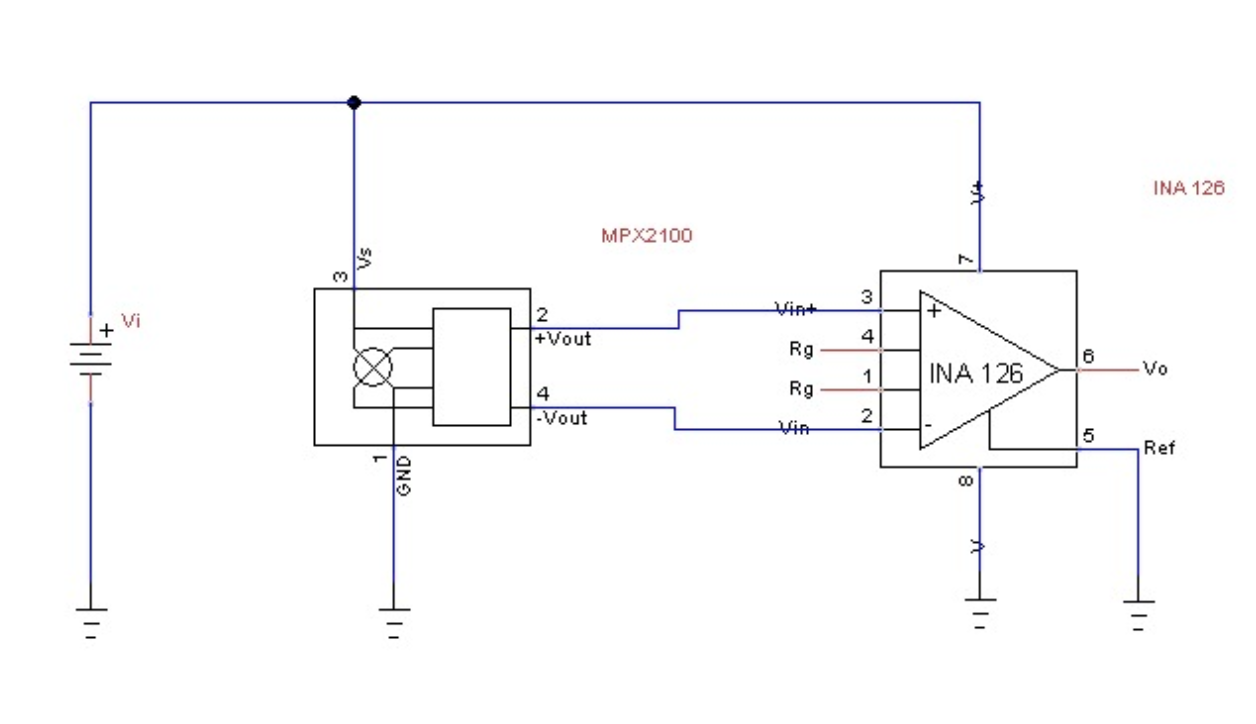
\includegraphics[width=105mm]{CirquitWP3.png}
		\end{center}
	\end{figure}
	
	\newpage
	\textcolor{blue}{Question 3.12:} \textbf{Obtain in the lab 10 measurement points along the measurement range. Draw its graphical representation, calculate and plot the linear regression and the linearity error (lineal regression straight line – measured points). }
	
	\begin{table}[H]
	\centering
	\begin{tabular}{||c c ||} 
	 \hline
		 Preassure[Atm] & Voltage[$V$] \\ [0.5ex] 
	 \hline\hline
	 	0 		& 1.96 \\
		 0.1 		& 1.97  \\ 
		 0.15 	& 1.98  \\ 
		 0.2 		&  1.99\\
		 0.25 	& 1.995  \\ 
		 0.3 		& 2.00 \\
		 0.35 	& 2.003  \\ 
		 0.4 		& 2.01 \\
		 0.45 	& 2.013  \\ 
		 0.5 		& 2.019 \\ [1ex] 
	 \hline
	\end{tabular}
	\caption{Voltage output respect to Preassure input}
	\end{table}
	
	
	\begin{figure}[H]
		\begin{center}
		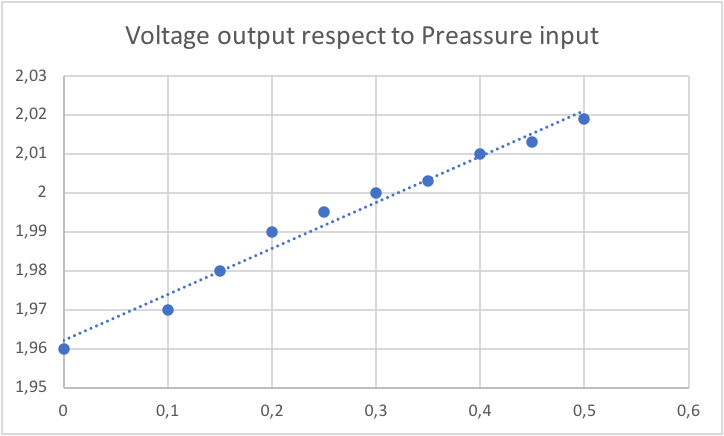
\includegraphics{ExcelGraph2.png}
		\end{center}
	\end{figure}
	
	\begin{figure}[H]
		\begin{center}
		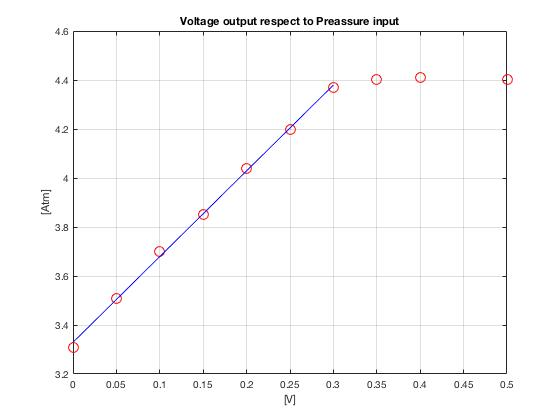
\includegraphics[width=105mm]{MatlabGraph1.jpg}
		\end{center}
	\end{figure}
	
	\lstinputlisting{codiMatlab.m}
	

	\textcolor{blue}{Question 3.13:}  \textbf{Calculate the digital data range provided by the acquisition circuit in measurements from 0 to 3m of water depth. Consider that the 10 bit A/D converter of the Arduino assigns 0 to a 0V input and 1023 (210-1) to a 5V input.}
	
	The expected values from the arduino measurement acquisition should be inside the interval
	\[
		[\frac{V_0}{5}\cdot1023, \frac{V_{0.3}}{5}\cdot1023] = [\frac{1.96}{5}\cdot1023, \frac{2.00}{5}\cdot1023] = [401.0,409.2]
	\]
	
	\textcolor{blue}{Question 3.14:} \textbf{Explain briefly what is the purpose of the following functions, used in the sketch of Fig. 4.5: Serial.begin(), analogRead(), Serial.println() and delay(). }
	\begin{itemize}
		\item \textbf{Serial.begin():} Sets the data rate in bits per second for serial data transmission.
		\item \textbf{analogRead():} Reads the value from the specified analog pin.
		\item \textbf{Serial.println():} Prints data to the serial port and skip the line.
		\item \textbf{delay():} Pauses the program for the amount of time specified as parameter.
	
	\end{itemize}


	\textcolor{blue}{Question 3.15:}  \textbf{While acquiring measures with the Arduino, smoothly increase the pressure to simulate a depth change from 0 m to 3 m. Do the measurement results displayed on the serial monitor match with the theoretical ones obtained in Question 3.13? If not, explain why. NOTE: If you are at home, use the potentiometer or the temperature sensor instead of the pressure sensor.}

	\begin{table}[H]
	\centering
	\begin{tabular}{||c c ||} 
	 \hline
		 Preassure[Atm] & Arduino output \\ [0.5ex] 
	 \hline\hline
	 	 0 		& 391  \\
		 0.1 		& 392  \\ 
		 0.15 	& 392  \\ 
		 0.2 		& 393  \\
		 0.25 	& 394  \\ 
		 0.3 		& 395  \\
		 0.35 	& 396  \\ 
		 0.4 		& 397  \\
		 0.45 	& 399  \\ 
		 0.5 		& 399  \\ [1ex] 
	 \hline
	\end{tabular}
	\caption{Arduino output respect to Preassure input}
	\end{table}
	
	FALTA EXPLICAR PERQUE NO ES IGUAL A LA PREGUNTA 3.13\\

	\textcolor{blue}{Question 3.16:} \textbf{Include a picture of the initial and final Gantt diagrams of WP3, making a reflexion about the progress and explaining any delay in the development of the tasks. }
	
	\begin{figure}[H]
		\begin{center}
		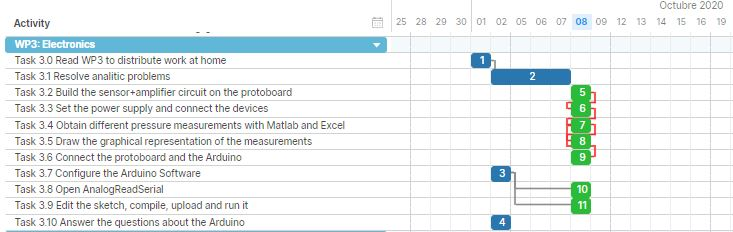
\includegraphics[width=150mm]{WP3-8-10-2020.jpg}
		\end{center}
	\end{figure}
	
	We completed the work in time because everything turned out as planned. We distributed the questions among the members before going to the lab and, once there, we knew exactly what to do and could benefit from the two hours to finish all the practical tasks. 
	
	\section{WP4 - Communications}
	
	\textcolor{blue}{Question 4.1:} \textbf{Encode in plain binary (2 bytes) the following measured value: 663. Determine the pressure corresponding to this value.}
	
	We can see that $663_{10} = (2^0 + 2^1 + 2^2 + 2^5 + 2^8)_{10} = 10010111_2$

	\textcolor{blue}{Question 4.2:}  \textbf{Encode in ASCII the following measurement data: 25, 663, 1012.}
	
		25: 50 53\\
		663: 54 54 51\\
		1012: 49 48 49 50\\
	\textcolor{blue}{Question 4.3:} \textbf{Go to the Arduino language reference and identify which types are suitable to work with the numeric data provided by the A/D converters. What code length (in bytes) corresponds to each type?}

	\textcolor{blue}{Question 4.4:} \textbf{Compare the screen captures obtained and explain the differences found. What sequence of bytes is really sent in each case?}

	\textcolor{blue}{Question 4.5:}  \textbf{List the serial port(s) COMx available in your computer. }
		In our computer we have COM1, COM7 and COM30 (which is the arduino one)
	\textcolor{blue}{Question 4.6:}  \textbf{Identify the cables color connected at the RS-232 send and receive pins.}

	\textcolor{blue}{Question 4.7:}  \textbf{Calculate which time-base must be selected in the oscilloscope to see 10 bits on the screen at the transmission rate selected by default in Terminal. }

	\textcolor{blue}{Question 4.8:} \textbf{Capture the waveform displayed on the oscilloscope. Determine the voltage levels, bit period and the number of bits per character. Which level indicates the idle state? Using an ASCII table explain the waveforms displayed for 3 different characters.}

	\textcolor{blue}{Question 4.9:} \textbf{What is the reason to use RS-232 to communicate with the ROUV, instead of using USB (which is available in both the Arduino and the computer)?}

	\textcolor{blue}{Question 4.10:} \textbf{Capture the waveform displayed on the oscilloscope. Obtain the voltage levels of the signal. Which level corresponds to the idle state?}

	\textcolor{blue}{Question 4.11:} \textbf{Draw the schematic (using the CAD schematic software https://www.tinycad.net/.) of the level shifter circuit, including only the transmission path (from the Arduino Tx pin to the RS-232 DB9-female connector). What are the appropriate values of capacitors C1, C2, C3 and C4?}

	\textcolor{blue}{Question 4.12:} \textbf{Describe the difference(s) between the sketches of Figs. 4.1 and 4.3 seen from the user.}

	\textcolor{blue}{Question 4.13:} \textbf{Explain why the Rx input pin of the Arduino must be in high impedance state (i.e. not connected) when a compiled sketch is being uploaded. }

	\textcolor{blue}{Question 4.14:} \textbf{Modify the sketch ENTIC-Analog2Serial-bidir to stop data sampling \& transmission when any of the following conditions is true: 1) timeout, i.e. data values must be sent for only 2 minutes; 2) end command from user, i.e. the Arduino receives the character ‘E’.  }


	\textcolor{blue}{Question 4.15:} \textbf{Explain and justify where these three components should be placed in Fig. 4.5: }
	
	a)  The resistor setting the amplifier gain (see WP3).
	
	b)  The jumper for the serial reception path (see Fig. 4.2).
	
	c)  The protection diode for the Arduino power input (see Fig. 4.4).

	\textcolor{blue}{Question 4.16:} \textbf{Using Fig. 4.5 as floorplan, draw a schematic describing how the circuits must be implemented on the interface-PCB. Identify and label all interconnection signals with the Arduino and the base PCBs (strip pins \& sockets), describe the placement of all electronic components and add cables whenever additional connections were necessary. Use a colour code to improve the readability and usefulness of the schematic (i.e. red for power supply tracks \& cables, black for GND, etc.)}

	\textcolor{blue}{Question 4.17:} \textbf{Include a picture of the initial and final Gantt diagrams of WP4, making a reflexion about the progress and explaining any delay in the development of the tasks.  }

	Bones 
	Molt bones
\end{document}